
\procTitle{Изменения биологических показателей основных промысловых видов камбал: звёздчатой (\textit{Platichthys stellatus}),
желтопёрой (\textit{Limanda aspera}), жёлтобрюхой (\textit{Pleuronectes quadrituberculatus}), обитающих в северной части Охотского моря }

\procAuthorI{Бурлак~Ф.\,А.}
\procEmailI{Ozzy38@yandex.ru}
\procOrganizationI{МагаданНИРО}
\procCityI{Магадан}

\procAuthorII{Смирнов~А.\,А.}
\procEmailII{andrsmir@mail.ru}
\procOrganizationII{ВНИРО}
\procCityII{Москва}
\procOrganizationIV{СВГУ}
\procCityIV{Магадан}

\makeProcTitleIVRazdel
\index{b@Бурлак~Ф.\,А.}
\index{s@Смирнов~А.\,А.}



В последние годы в северной части Охотского моря активно развивается промысел донных рыб [2], в том числе и прибрежный лов камбал. Дальневосточные камбалы, как и~в~других районах дальневосточного бассейна, в северной части Охотского моря служат основой развития прибрежного рыболовства [4].

В настоящее время прибрежный промысел камбал в северной части Охотского моря базируется на трёх основных видах: желтопёрой (\textit{Limanda aspera}), звёздчатой (\textit{Platichthys stellatus}) и жёлтобрюхой (\textit{Pleuronectes quad\-ri\-tu\-ber\-culatus}).

Желтопёрая камбала является видом, на котором базируется промысел камбал в рассматриваемом районе. Её доля в уловах, по нашим данным, составляет 95,6~\% от общего вылова. Она является прибрежным видом, достигающим длины 49~см (в основном преобладают особи длиной 19--35~см), образуя максимальные скопления в нерестовый период на глубинах 20--40~м. Нерестится с конца мая по сентябрь, в июле нерест достигает массового развития [3].

Звёздчатая камбала в северной части Охотского моря начинает нереститься в мае~--- июне. Максимальный размер составляет 58,5~см в возрасте 23+~лет [5]. Достаточно многочисленный вид, уступающий по численности только желтопёрой камбале, который в отдельных частях Охотского моря может составить до 51\,\% от общего вылова камбал [3].

Самки жёлтобрюхой камбалы в северной части Охотского моря в возрасте 24+ лет могут достигать 62,5~см [5]. Зимой эта камбала образует скопления на глубинах около 300~м, а~летом~--- на глубинах менее 100~м [3]. На прибрежном промысле встречается в единичных экземплярах. Достаточно часто штучно наблюдается при промысле минтая в летний период.

На рис. 1--4 показана межгодовая динамика средних биологических показателей (размер, масса, возраст, доля самок) для таких видов, как желтопёрая (\textit{Limanda aspera}), жёлтобрюхая (\textit{Pleuronectes quadrituberculatus}) и~звёздчатая (\textit{Platichthys stellatus}) камбалы из~исследовательских уловов МагаданНИРО. Лов проводили ставными сетями в мае~--- июле 2007--2019~гг.
\clearpage
\begin{figure}[h!]
  \begin{center}
    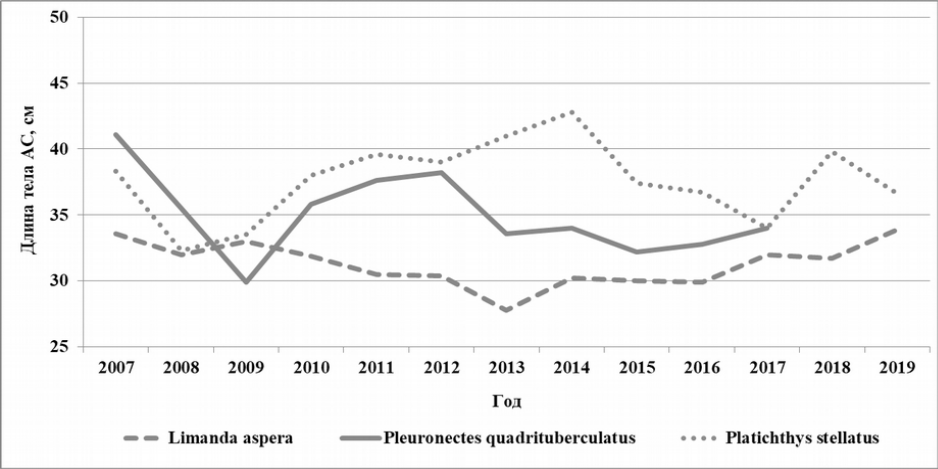
\includegraphics[width=0.9\textwidth]{authors/Byrlak-fig1.png}
  \end{center}
  \caption{Динамика средней длины тела АС (см) камбал из исследовательских уловов в северной части Охотского моря}
  \label{fig:byrlak-fig1}
\end{figure}

\begin{figure}[h!]
  \begin{center}
    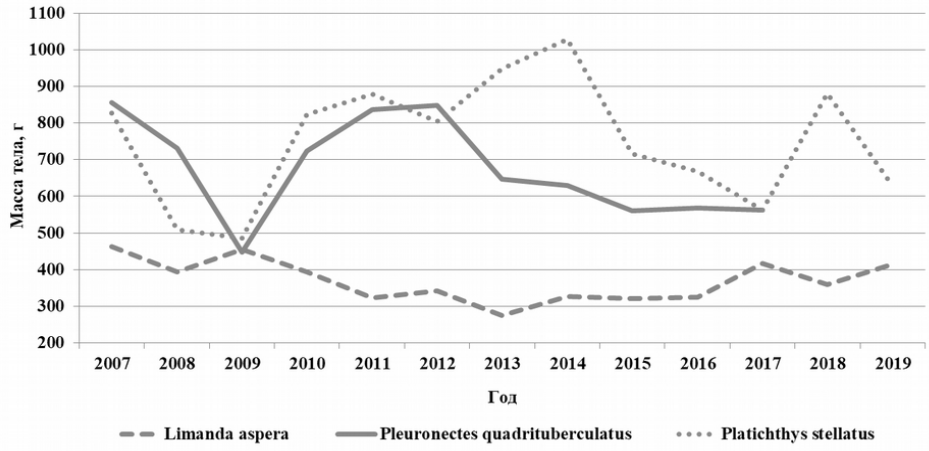
\includegraphics[width=0.9\textwidth]{authors/Byrlak-fig2.png}
  \end{center}
  \caption{Динамика средней массы тела (г) камбал из исследовательских уловов в~северной части Охотского моря}
  \label{fig:byrlak-fig2}
\end{figure}

\begin{figure}[h!]
  \begin{center}
    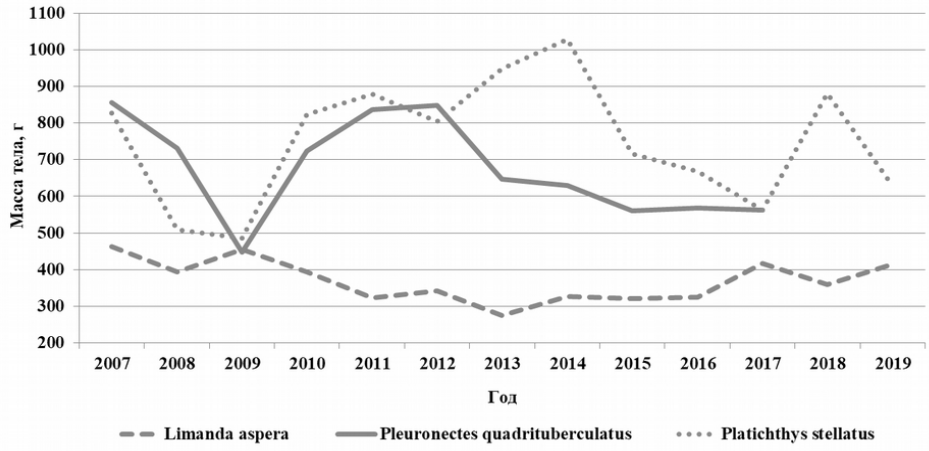
\includegraphics[width=0.9\textwidth]{authors/Byrlak-fig2.png}
  \end{center}
  \caption{Динамика среднего возраста (лет) камбал из исследовательских уловов в~северной части Охотского моря}
  \label{fig:byrlak-fig3}
\end{figure}

\begin{figure}[h!]
  \begin{center}
    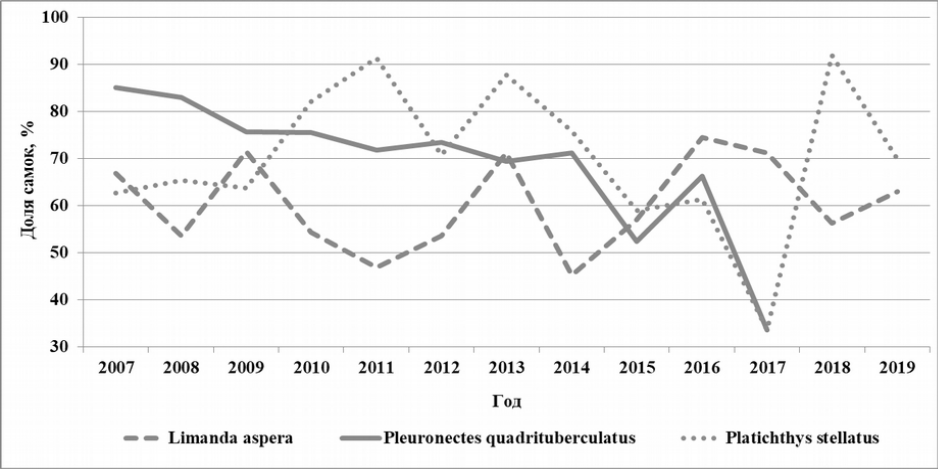
\includegraphics[width=0.9\textwidth]{authors/Byrlak-fig4.png}
  \end{center}
  \caption{Динамика доли самок камбал из исследовательских уловов в северной части Охотского моря}
  \label{fig:byrlak-fig4}
\end{figure}


В динамике средней длины и массы тела желтопёрой камбалы (рис.~1, 2) в последние годы видим незначительный подъём показателей, возможно, связанный с увеличением доли самок в уловах (рис. 4), которые крупнее самцов [1]. В то же время наблюдается снижение значения среднего возраста рыб (рис. 3).

Жёлтобрюхая камбала в исследовательских уловах 2018 и 2019~г. не~наблюдалась. Начиная с 2012~г. фиксируется снижение средних биологических показателей, таких как размер, масса и доля самок (рис. 1, 2, 4).
\clearpage
У звёздчатой камбалы происходит возрастание доли самок и снижение среднего возраста рыб (рис. 3, 4), что косвенно может являться индикатором вступления в промысел урожайного (высокочисленного) пополнения, поскольку пресс промысла на этот объект не~значителен.

В целом за период активного промышленного лова, в последние годы в~уловах, по нашим данным, наблюдаются скачки в средних биологических показателях для всех исследуемых видов камбал. Периодическое появление в уловах значительного количества мелких особей может свидетельствовать, с одной стороны, о чрезмерном прессе промысла, а с другой~--- о~возможном урожайном (высокочисленном) пополнении. Данные предположения нуждаются в дополнительных подтверждениях по результатам комплексных донных съёмок, которые необходимо выполнять в периоды различной активности рыб.

Поскольку промысел камбал приурочен к лету (в период большей пищевой и нерестовой активности), следует учитывать и такой фактор, как их слабая миграционная активность. Ошибочным будет мнение о~повсеместной большой плотности камбал в данный период, поскольку нерестовые и нагульные скопления локализированы только на определённых акваториях. За~2015--2019~гг. суммарный среднегодовой вылов желтопёрой (которая доминирует в уловах), жёлтобрюхой и звёздчатой камбал составил 165,2\,\% от рекомендуемого, при колебаниях от 76,6\,\% в 2015~г. до 300,7\,\% в 2019~г.


Такой чрезмерный вылов камбал, который в последние годы локализирован в небольших районах Тауйской губы и примыкающих к ней участках Притауйского района, до зал.~Бабушкина, может негативно сказаться на состоянии численности и биомассы этих видов в~целом.


\begin{thebibliography}{99}

\bibitem{}
\BibAuthor{Дьяков~Ю.\,П.} Размерно-половая и половозрастная структура популяций дальневосточных камбал // Известия ТИНРО.~--- 2014.~--- Т.~177.~--- С.~78--109.
\bibitem{}
\BibAuthor{Семёнов~Ю.\,К., Смирнов~А.\,А., Елатинцева~Ю.\,А., Ткаченко~А.\,А.} Особенности промысла донных рыб в 2019~г. в северной части Охотского моря // Рыбное хозяйство.~--- 2020.~--- №~2.~--- С.~43--50.
\bibitem{}
\BibAuthor{Черешнев~И.\,А., Волобуев~В.\,В., Хованский~И.\,Е., Шестаков~А.\,В.} Прибрежные рыбы северной части Охотского моря.~--- Владивосток~: Дальнаука, 2001.~--- 197~с.
\bibitem{}
\BibAuthor{Юсупов~Р.\,Р. и др.} Структура улова, состояние и промысел донных рыб в Северо-Охотоморском промысловом районе и зал. Шелихова Охотского моря / авт. Р.\,Р.~Юсупов, Ю.\,К.~Семёнов, Л.\,П.~Николенко, А.\,И.~Каика, М.\,В.~Ракитина, А.\,С.~Сергеев, А.\,Ю.~Немченко, Ю.\,В~Сидяков  / Отчётная сессия ФГУП <<МагаданНИРО>> по результатам научных исследований 2011~г.~: материалы докладов.~--- Магадан~: МагаданНИРО, 2012.~--- С.~103--107.
\bibitem{}
\BibAuthor{Юсупов~Р.\,Р., Семёнов~Ю.\,К., Шилин~Ю.\,А.} Рост и продукция массовых видов камбаловых рыб (Pleuronectidae) северной части Охотского моря // Исследования водных биологических ресурсов Камчатки и северо-западной части Тихого океана~: сб. науч. тр. Камчат. НИИ рыб. хоз-ва и океанографии.~--- 2015.~--- Вып.~36.~--- С.~14--24.
\end{thebibliography}
